\documentclass[conference]{IEEEtran}
\IEEEoverridecommandlockouts
\usepackage{cite}
\usepackage{amsmath,amssymb,amsfonts}
\usepackage{graphicx}
\graphicspath{{../figures/}}
\usepackage{textcomp}
\usepackage{xcolor}
\usepackage{booktabs}
\usepackage{url}
\usepackage{xurl}
\usepackage{iftex}
\ifXeTeX\usepackage{fontspec}\setmainfont{texgyretermes}[Extension=.otf,UprightFont=*-regular,BoldFont=*-bold,ItalicFont=*-italic,BoldItalicFont=*-bolditalic]\fi
\begin{document}

\title{Architectural Implementation of Neural Additive Models via Discrete Step Activations for Clinical Guideline Alignment}

\author{\IEEEauthorblockN{Pranav Mamidala}
\IEEEauthorblockA{Monta Vista High School, Cupertino, California, USA\\
\texttt{prnvmamidala@gmail.com}}}

\maketitle

\begin{abstract}
Often, machine learning models for early-warning prediction are not practical in the clinical setting because they lack interpretability and transparency, which blocks many providers from trusting the prediction process. One of the main reasons is that smooth neural networks learn continuous curves from continuous variables, while hospital guidelines use specific protocol cutoffs for risk assessment. We call this mismatch the continuous lab-value disconnect. Shock Index is one such example: values near 0.7 and 1.0 already guide escalation decisions, but a standard Neural Additive Model (NAM) may still return a gradual S-shaped risk curve. We hypothesized that by replacing the smooth Shock Index pathway with a hard step activation tied to clinically motivated thresholds, we could force complete step alignment with similar observed discrimination. We evaluated this as retrospective risk classification on three real public cohorts: prevalent self-reported cardiovascular disease history in NHANES ($n{=}6979$) and in-hospital mortality in PhysioNet 2012 ICU ($n{=}11520$) and the eICU demo ($n{=}1929$). Across five paired splits, the step-activation NAM had held-out AUROC within 0.01 of a vanilla Tanh NAM (0.7828 vs.\ 0.7838, 0.6303 vs.\ 0.6345, and 0.7421 vs.\ 0.7517) and was similar to a binned logistic regression with an age spline (0.7815, 0.6312, and 0.7418). The constrained Shock Index contribution was exactly piecewise constant, with jumps only at 0.7 and 1.0, and its learned levels increased monotonically in every cohort and run, although the architecture itself does not guarantee this ordering.
\end{abstract}

\begin{IEEEkeywords}
Neural Additive Models, Shock Index, step activation, clinical guidelines, interpretability, primary care setting
\end{IEEEkeywords}

\section{Introduction}
Despite significant advances in AI, many early-warning models remain difficult to adopt in the primary care setting, mainly because they lack interpretability.~\cite{rudin2019} Tabular early-warning systems are central to the intensive care unit (ICU) and emergency workflows for shock and related circulatory failure, where early detection matters for rapid treatment to prevent harm.~\cite{allgower1967,koch2019} Machine learning has been shown to be a useful tool for risk prediction, but many models maximize precision through complex architectures, often sacrificing practicality in the clinical setting.

Neural Additive Models (NAMs) hold great promise because each feature has its own sub-network and the final prediction is an additive combination of those contributions, so each pathway can be plotted and inspected.~\cite{agarwal2021} This inspectability and interpretability is valuable for clinical AI, but it does not automatically produce explanations that match hospital protocols. The core conflict is that NAMs trained with smooth activations typically learn continuous curves from raw data frequencies, whereas clinicians operate on discrete and deterministic protocol cutoffs. For Shock Index, defined as heart rate divided by systolic blood pressure, values near 0.7 and 1.0 are commonly used as clinically motivated cutoffs in the literature.~\cite{allgower1967,koch2019} Allg\"{o}wer and Burri described a normal Shock Index of roughly 0.5 to 0.7,~\cite{allgower1967} and emergency department studies reviewed by Koch \textit{et al.} associate values above about 1.0 with worse outcomes,~\cite{koch2019} although these are not universal operational cutoffs used by every hospital. A smooth NAM may assign a slightly different risk contribution at Shock Index 0.71 versus 0.69 even when both values fall on the same side of a protocol boundary, which can make the explanation feel clinically inconsistent.

We hypothesized that an architectural modification, switching the smooth Shock Index pathway for a discrete threshold switch, could produce guideline-aligned explanations without complex hyperparameter-sensitive derivative penalties. Related approaches try to reshape learned curves after the fact with regularization, but those methods introduce extra loss terms and burden. This study instead modifies the model structure so that non-guideline curvature is impossible on the Shock Index pathway. We compare a vanilla Tanh NAM against a structurally constrained step-activation NAM trained with standard binary cross-entropy only, and against binned logistic regression baselines that use the same Shock Index bands.

\section{Methodology and Mathematical Framework}
A key requirement of this study was to keep the model clinically relevant without sacrificing a clear link between Shock Index and protocol cutoffs.

\subsection{Neural Additive Model}
Let $x_{\mathrm{SI}}$ denote Shock Index and $x_{\mathrm{Age}}$ denote age. A two-feature NAM predicts event risk as
\begin{equation}
\hat{p}(x)=\sigma\bigl(f_{\mathrm{SI}}(x_{\mathrm{SI}})+f_{\mathrm{Age}}(x_{\mathrm{Age}})\bigr),
\label{eq:nam}
\end{equation}
where $\sigma$ is the logistic sigmoid and $f_{\mathrm{SI}}$ and $f_{\mathrm{Age}}$ are feature-specific contribution functions. Because the pathways do not mix, $f_{\mathrm{SI}}$ is an explicit shape function that can be plotted independently of age. This is what makes NAMs suitable for clinical audit in which a reviewer can ask how Shock Index alone moves predicted risk while holding age fixed in the additive sense of~\eqref{eq:nam}.

\subsection{Vanilla Smooth Pathway}
In the vanilla NAM, both sub-networks use the same multilayer architecture,
\begin{equation}
1\rightarrow 64\rightarrow 64\rightarrow 1,
\label{eq:mlp}
\end{equation}
with $\tanh$ hidden activations and a linear output. This design can represent flexible continuous curves and is a strong baseline for predictive accuracy. However, it has no knowledge that clinicians treat 0.7 and 1.0 as special boundaries, so the learned Shock Index shape can place slope anywhere in the domain.

\subsection{Hard Step Activation for Shock Index}
In the threshold-constrained NAM, the age pathway remains a Tanh multilayer network identical to the vanilla age pathway, while the Shock Index pathway is replaced by a hard step activation with three learnable levels $b_0,b_1,b_2$:
\begin{equation}
f_{\mathrm{SI}}(x)=
\begin{cases}
b_0, & x<0.7,\\
b_1, & 0.7\le x<1.0,\\
b_2, & x\ge 1.0.
\end{cases}
\label{eq:step}
\end{equation}
Using boolean indicators,
\begin{equation}
\begin{aligned}
f_{\mathrm{SI}}(x)
&= b_0\cdot\mathbf{1}\{x<0.7\} + b_1\cdot\mathbf{1}\{0.7\le x<1.0\}\\
&\quad + b_2\cdot\mathbf{1}\{x\ge 1.0\}.
\end{aligned}
\label{eq:masks}
\end{equation}
Equation~\eqref{eq:masks} is integrated with boolean masks instead of approximations so the contribution is exactly the same within each clinical band and can change only at the guideline thresholds. The parameters $b_0,b_1,b_2$ are ordinary neural network weights. During training, backpropagation updates only the active level for each sample, while the age network continues to learn a smooth contribution.

This constraint in architecture explicitly restricts the Shock Index output space to a three-level step function. Both models use the same binary cross-entropy objective and the Adam optimizer. Alignment with the predefined cutoffs is made by structure. The proposed architecture guarantees piecewise-constant Shock Index contributions at predefined thresholds, but does not independently guarantee monotonic risk contributions, clinical validity, or patient safety. In this way, a bedside reviewer can verify the Shock Index pathway by reading three numbers and two cutoffs, rather than inspecting a continuous curve for accidental slope in safe zones.

\subsection{Clinical Cohorts and Training Protocol}
We used three public cohorts that can be downloaded without credentials. \textit{NHANES:} adults aged 20 or older in the 2017 to March 2020 pre-pandemic cycle,~\cite{nhanes} with Shock Index taken from the first oscillometric pulse and systolic blood pressure. The label was self-reported prior cardiovascular disease (heart failure, coronary heart disease, angina, heart attack, or stroke), giving $n{=}6979$ and a prevalence of 12.2\%. \textit{PhysioNet 2012:} ICU stays from sets A, B, and C of the PhysioNet/CinC Challenge 2012,~\cite{silva2012,goldberger2000} with Shock Index from the first time-matched heart rate and systolic blood pressure in the first 6 hours (non-invasive preferred). The label was in-hospital death, giving $n{=}11520$ and a prevalence of 14.2\%. \textit{eICU demo:} the first ICU stay of each adult hospital admission in the eICU-CRD demo,~\cite{pollard2018} with the first systolic blood pressure in the first 6 hours paired with the heart rate closest in time (within 15 minutes). The label was hospital death, giving $n{=}1929$ and a prevalence of 8.8\%. In both ICU cohorts, vitals come only from the start of the stay, so they precede the outcome. Fig.~\ref{fig:data} shows the observed event rate by Shock Index bin in each cohort. The number of patients below 0.7, between 0.7 and 1.0, and at or above 1.0 was 5833/1118/28 for NHANES, 5246/4701/1573 for PhysioNet 2012, and 915/706/308 for the eICU demo.

For each seed from 0 to 4, we drew one stratified 80/20 train/test split, and the seed also set the initialization. Every model was trained on the same 80\% and scored once on the same held-out 20\% test set, so differences between models are paired by split. There was no separate validation set, because nothing was selected on held-out data: all models were trained for 150 epochs with Adam (learning rate $10^{-3}$, batch size 64) using binary cross-entropy with logits. No warm-start schedule and no penalty ramp were used for the constrained model, because the step structure is present from initialization. Hyperparameters were fixed in advance and carried over from our earlier experiment, with no early stopping. We report Mean$\pm$SD over the five seeds. As baselines, we fit (a) a binned logistic regression with one-hot Shock Index bands ($<0.7$, $0.7$ to $1.0$, $\ge1.0$) and a linear age term, and (b) the same bands with a cubic age spline (5 knots), both with L2 penalty $C{=}1$. Because \eqref{eq:masks} is equivalent to one-hot bands, baseline (b) closely reproduces the functional form of the step NAM without a neural network. For cutoff sensitivity, we retrained the step NAM with cutoffs (0.6, 0.9) and (0.8, 1.1) on the same splits. All numbers below come from the executed scripts in \url{https://github.com/prnvmamidala-cmd/Neural-Additive-Models-Step-Constraint-for-Clinical-Application}.

\section{Experimental Results and Discussion}

\subsection{Discrimination}
Across five seeds, held-out test AUROC was $0.7838\pm0.0206$ for the vanilla NAM and $0.7828\pm0.0208$ for the hard step-activation NAM on NHANES, $0.6345\pm0.0141$ versus $0.6303\pm0.0176$ on PhysioNet 2012, and $0.7517\pm0.0320$ versus $0.7421\pm0.0283$ on the eICU demo (Table~\ref{tab:auroc}). Brier scores were also close (0.0964 versus 0.0964, 0.1184 versus 0.1187, and 0.0725 versus 0.0742). The paired AUROC difference (vanilla minus step) was $+0.0010$ (95\% CI $-0.0031$ to $0.0052$), $+0.0042$ ($-0.0027$ to $0.0111$), and $+0.0097$ ($-0.0103$ to $0.0296$), using a $t$-interval over the five splits. These intervals include zero, so replacing the smooth Shock Index pathway with a discrete step activation gave similar observed discrimination on these cohorts. They do not establish equivalence, and the eICU interval is wide enough that a loss of up to about 0.03 cannot be ruled out.

The binned baselines performed about the same as the step NAM. Binned logistic regression with an age spline reached $0.7815\pm0.0209$, $0.6312\pm0.0153$, and $0.7418\pm0.0357$, with paired differences versus the step NAM of $-0.0012$ ($-0.0028$ to $0.0004$), $+0.0008$ ($-0.0025$ to $0.0042$), and $-0.0003$ ($-0.0214$ to $0.0208$). This is expected, since the step pathway is a one-hot discretization. The value of our approach is therefore not higher accuracy than ordinary discretization, but a transparent implementation of guideline discretization inside the NAM structure, so the same model family can mix constrained and smooth pathways and still be read pathway by pathway.

\begin{table}[!t]
\caption{Held-out test AUROC and Brier score (Mean$\pm$SD over seeds 0 to 4, same splits for all models).}
\begin{center}
\footnotesize\setlength{\tabcolsep}{1.6pt}
\begin{tabular}{lccc}
\toprule
\textbf{Model} & \textbf{NHANES} & \textbf{PhysioNet 2012} & \textbf{eICU demo} \\
\midrule
\multicolumn{4}{l}{\textit{AUROC}} \\
Vanilla NAM & $0.784\pm0.021$ & $0.635\pm0.014$ & $0.752\pm0.032$ \\
Hard Step NAM & $0.783\pm0.021$ & $0.630\pm0.018$ & $0.742\pm0.028$ \\
Binned LR & $0.782\pm0.021$ & $0.629\pm0.016$ & $0.746\pm0.034$ \\
Binned LR + spline & $0.782\pm0.021$ & $0.631\pm0.015$ & $0.742\pm0.036$ \\
\midrule
\multicolumn{4}{l}{\textit{Brier score}} \\
Vanilla NAM & $0.0964\pm0.0015$ & $0.1184\pm0.0012$ & $0.0725\pm0.0033$ \\
Hard Step NAM & $0.0964\pm0.0026$ & $0.1187\pm0.0007$ & $0.0742\pm0.0019$ \\
Binned LR & $0.0956\pm0.0020$ & $0.1186\pm0.0008$ & $0.0738\pm0.0024$ \\
Binned LR + spline & $0.0955\pm0.0019$ & $0.1183\pm0.0008$ & $0.0741\pm0.0024$ \\
\bottomrule
\end{tabular}
\label{tab:auroc}
\end{center}
\end{table}

Fig.~\ref{fig:roc} shows that the ROC curves nearly overlap in all three cohorts, consistent with the small AUROC gap. This is consistent with the hard structural constraint giving similar ranking quality for the binary event label.

\begin{figure}[!t]
\centerline{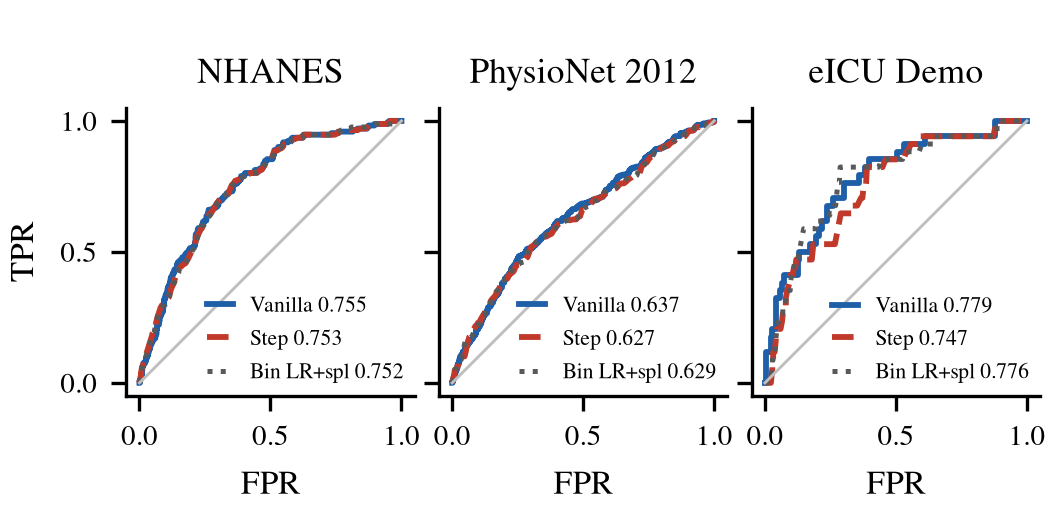
\includegraphics[width=\columnwidth]{fig_roc.png}}
\caption{Held-out test ROC curves (seed 0 split) for the vanilla NAM, hard step-activation NAM, and binned LR with age spline. Legends give AUROC.}
\label{fig:roc}
\end{figure}

\begin{figure}[!t]
\centerline{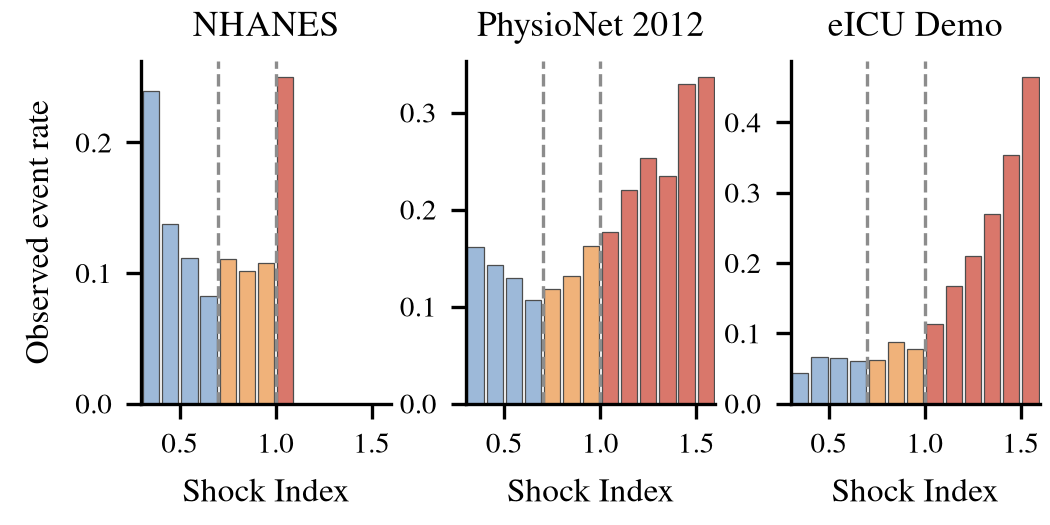
\includegraphics[width=\columnwidth]{fig_data_event_rate.png}}
\caption{Observed event rate by Shock Index bin in each cohort (bins with fewer than 15 patients omitted). Dashed lines mark clinical cutoffs at 0.7 and 1.0.}
\label{fig:data}
\end{figure}

\subsection{Shape Alignment}
Fig.~\ref{fig:shapes} plots centered Shock Index contributions. The vanilla NAM learns a smooth curve that spreads risk continuously across the domain and does not flatten between protocol cutoffs. The hard step-activation NAM is a clear piecewise constant: flat below 0.7, flat between 0.7 and 1.0, and flat at or above 1.0, with jumps only at the guideline boundaries. Averaged over seeds 0 to 4, learned raw step levels were $b_0=-0.187$, $b_1=0.269$, and $b_2=0.701$ on NHANES, $b_0=-0.252$, $b_1=-0.126$, and $b_2=0.517$ on PhysioNet 2012, and $b_0=-0.599$, $b_1=-0.222$, and $b_2=0.792$ on the eICU demo (Table~\ref{tab:steps}). These levels increased in a monotonic nature in every cohort and in all 15 runs at the 0.7 and 1.0 cutoffs, and they match the direction of the observed event rates in Fig.~\ref{fig:data}, where the largest rise occurs at or above 1.0. The constrained model therefore flattens within-band variation and concentrates all Shock Index meaning change into vertical steps at the exact clinical boundaries.

\begin{figure*}[!t]
\centerline{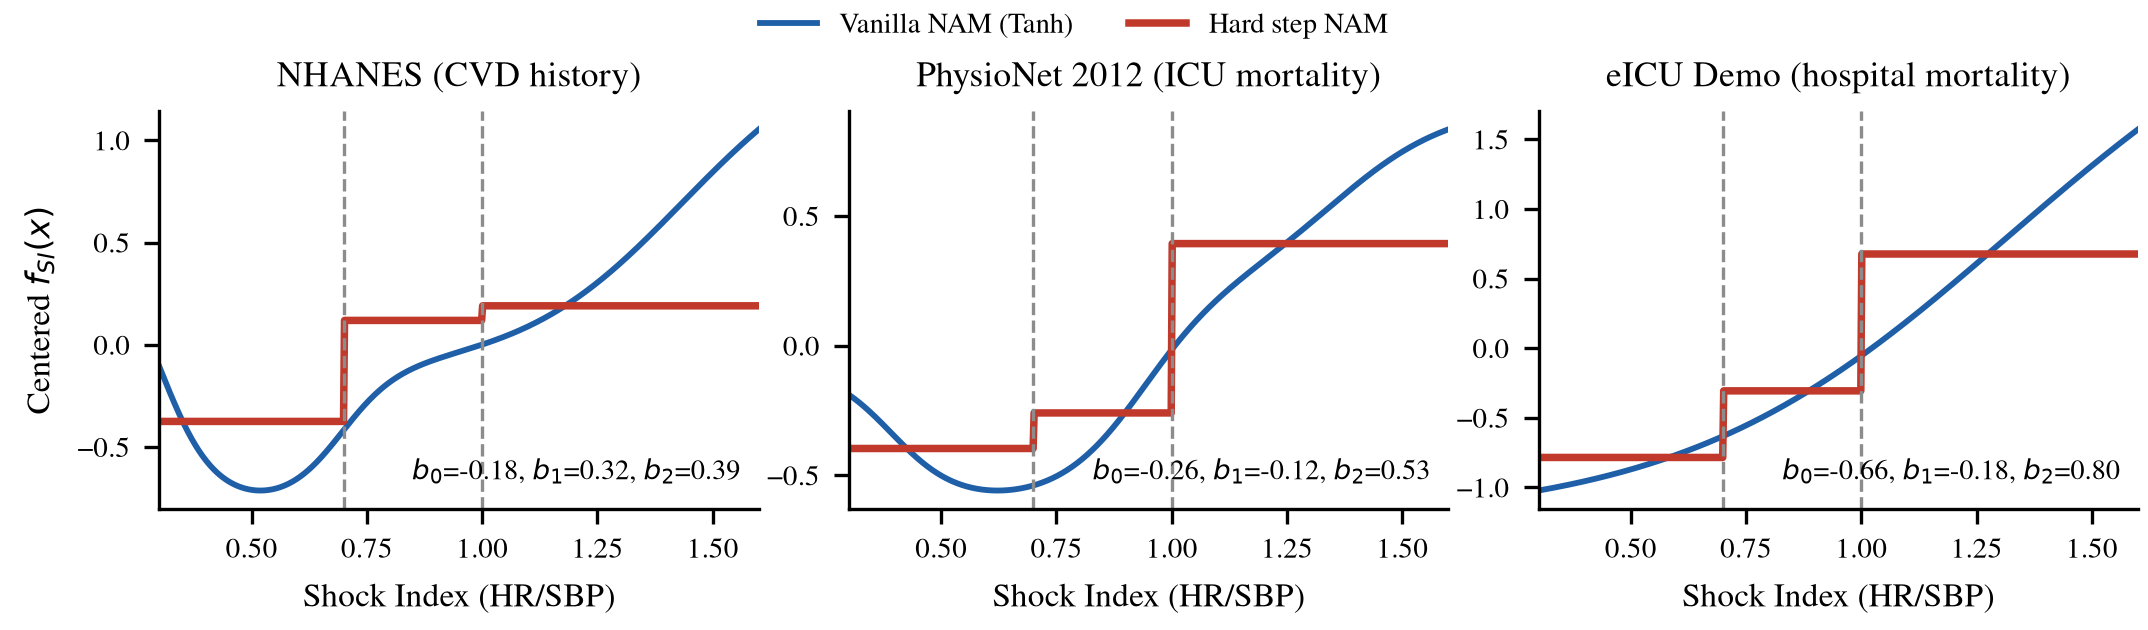
\includegraphics[width=0.95\textwidth]{clinical_step_activation_results.png}}
\caption{Learned Shock Index shape functions (seed 0 split). Blue: vanilla Tanh NAM. Red: hard step-activation NAM with jumps only at 0.7 and 1.0. Both models report similar AUROC under BCE-only training in each cohort.}
\label{fig:shapes}
\end{figure*}

\begin{table}[!t]
\caption{Learned Shock Index step levels in the constrained NAM (Mean over seeds 0 to 4).}
\begin{center}
\footnotesize\setlength{\tabcolsep}{3pt}
\begin{tabular}{llccc}
\toprule
\textbf{Region} & \textbf{Condition} & \textbf{NHANES} & \textbf{PhysioNet} & \textbf{eICU} \\
\midrule
Normal & $x_{\mathrm{SI}}<0.7$ & $b_0$: $-0.187$ & $-0.252$ & $-0.599$ \\
Elevated & $0.7\le x_{\mathrm{SI}}<1.0$ & $b_1$: $\phantom{-}0.269$ & $-0.126$ & $-0.222$ \\
Critical & $x_{\mathrm{SI}}\ge 1.0$ & $b_2$: $\phantom{-}0.701$ & $\phantom{-}0.517$ & $\phantom{-}0.792$ \\
\bottomrule
\end{tabular}
\label{tab:steps}
\end{center}
\end{table}

From a clinic-facing perspective, Table~\ref{tab:steps} is the explanation. A reviewer does not need to interpret a continuous spline-like curve because the Shock Index effect is summarized by three region levels and two protocol cutoffs already used in shock triage. That is the intended view of the continuous lab-value disconnect for this feature.

\subsection{Cutoff Sensitivity}
Table~\ref{tab:sens} reports the step NAM retrained with shifted cutoffs on the same splits. AUROC changed by at most 0.009 across cutoff pairs within any cohort, so discrimination was not very sensitive to the exact cutoffs. Monotonic levels were less stable. With (0.6, 0.9), $b_0$ exceeded $b_1$ in all five PhysioNet runs, matching the observed event rates of 13.9\% below 0.6 and 11.8\% between 0.6 and 0.9, and with (0.8, 1.1) one NHANES run was not monotonic, where only 8 participants fell at or above 1.1. This shows directly that monotonicity is an empirical property of the data and cutoffs, not of the architecture. This is a cutoff sensitivity analysis and does not test robustness when true risk is smooth.

\begin{table}[!t]
\caption{Cutoff sensitivity of the hard step NAM: test AUROC (Mean$\pm$SD), runs with $b_0<b_1<b_2$, and patients per band.}
\begin{center}
\footnotesize\setlength{\tabcolsep}{2.5pt}
\begin{tabular}{llccc}
\toprule
\textbf{Cutoffs} & & \textbf{NHANES} & \textbf{PhysioNet 2012} & \textbf{eICU demo} \\
\midrule
(0.6, 0.9) & AUROC & $0.779\pm0.021$ & $0.629\pm0.010$ & $0.733\pm0.031$ \\
 & Monotone & 5/5 & 0/5 & 5/5 \\
 & Bands & 4320/2564/95 & 3122/5765/2633 & 569/896/464 \\
(0.7, 1.0) & AUROC & $0.783\pm0.021$ & $0.630\pm0.018$ & $0.742\pm0.028$ \\
 & Monotone & 5/5 & 5/5 & 5/5 \\
 & Bands & 5833/1118/28 & 5246/4701/1573 & 915/706/308 \\
(0.8, 1.1) & AUROC & $0.781\pm0.021$ & $0.633\pm0.013$ & $0.738\pm0.032$ \\
 & Monotone & 4/5 & 5/5 & 5/5 \\
 & Bands & 6590/381/8 & 7284/3303/933 & 1206/530/193 \\
\bottomrule
\end{tabular}
\label{tab:sens}
\end{center}
\end{table}

\subsection{Training Behavior}
Fig.~\ref{fig:train} shows that both models trained stably under the same BCE objective. Train and held-out test losses decreased quickly and then stayed level over 150 epochs, and the constrained model did not require a separate penalty schedule. Because the step constraint is architectural, hyperparameter search was limited to normal optimizer settings shared with the vanilla baseline. This is a practical advantage over loss-based geometric penalties that can collapse shape quality when the penalty weight is set too aggressively.

\begin{figure*}[!t]
\centerline{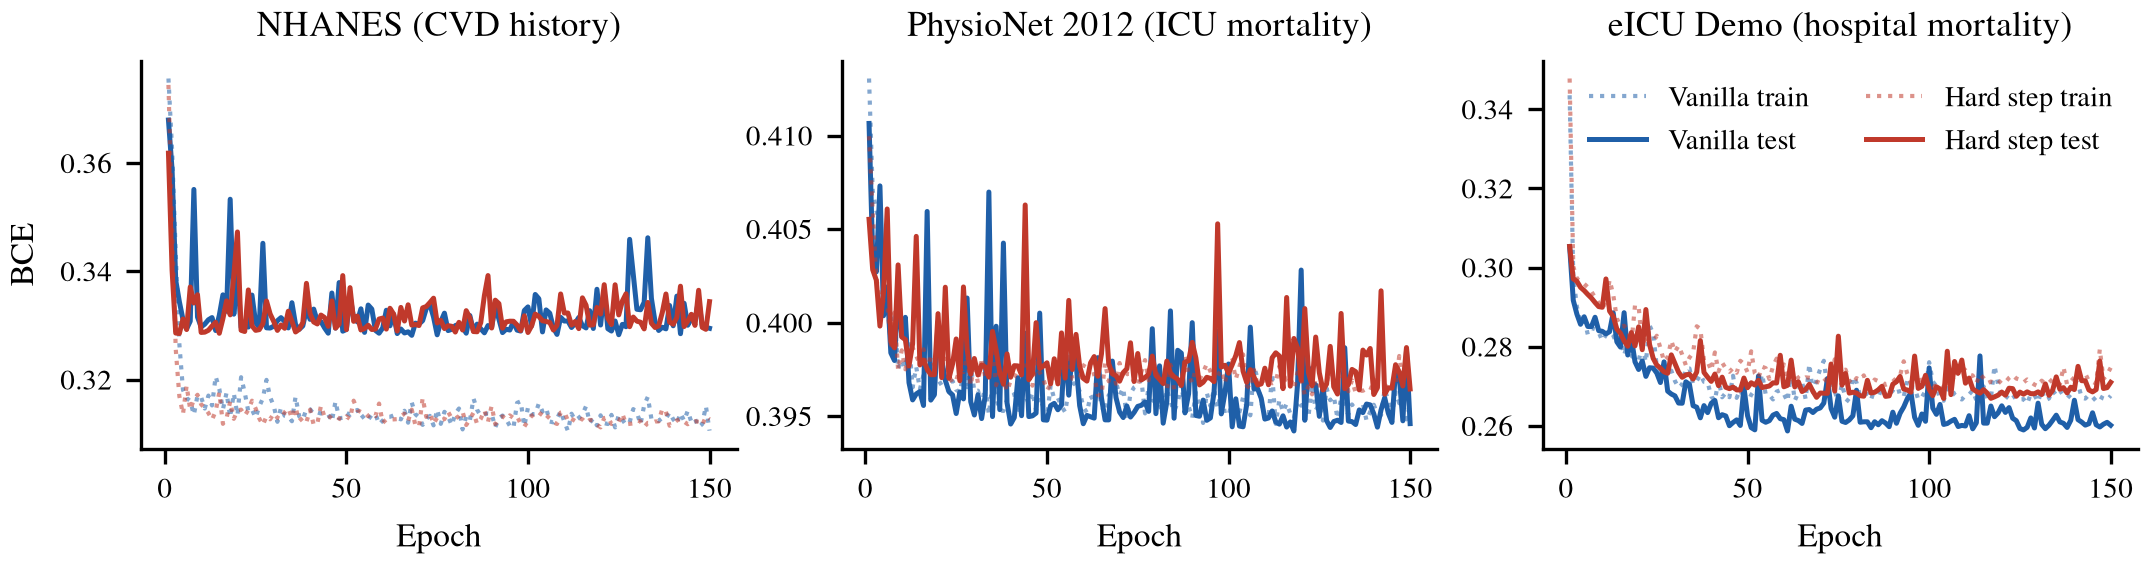
\includegraphics[width=0.95\textwidth]{fig_training_curves.png}}
\caption{Training curves (seed 0 split) for vanilla and hard step-activation NAMs under BCE only. Test BCE was logged for plotting only and was not used for stopping or selection.}
\label{fig:train}
\end{figure*}

\subsection{Limitations}
A limitation of our study is that real EHR labels are noisy, partially missing, and confounded, and our cohorts reflect this. The NHANES label is self-reported prior cardiovascular disease, not a future event, so NHANES results describe prevalent disease classification and not early warning, and only 28 NHANES participants had a Shock Index at or above 1.0, so $b_2$ is weakly identified there. NHANES also shows a higher event rate at the lowest Shock Index values, likely because of age and medication effects that a two-feature model cannot separate, and we did not apply survey weights. The 0.7 and 1.0 cutoffs come from the Shock Index literature and were not tuned for each cohort, and they may be less meaningful for resting survey vitals than for acute care. Discrimination on PhysioNet 2012 was modest for both models, since Shock Index and age alone carry limited mortality signal, and the eICU demo is small, which widens the spread across seeds. The step NAM did not outperform binned logistic regression with the same bands, so our contribution is interpretability through structural constraint and not predictive gain. Our confidence intervals come from only five splits. We evaluated two features only, five seeds, and a single snapshot of vitals per patient. Hard steps also reduce within-band flexibility, which may not be desirable when true risk varies in a smooth fashion within a protocol band. In that case, a softer constraint or additional within-band features may be needed. Our cutoff sensitivity analysis shifted both cutoffs together and did not test smooth true-risk scenarios, and we did not study whether cutoffs chosen by local hospital policy would transfer without changing $b_0,b_1,b_2$. Finally, the architecture does not guarantee monotonic levels, clinical validity, or patient safety, and our results are retrospective.

\section{Conclusion and Future Work}
We presented an architectural approach to clinical threshold alignment in NAMs: a hard step activation on the Shock Index pathway that implements literature-based Shock Index bands in an interpretable fashion. In retrospective risk classification on three real public cohorts, one for prevalent cardiovascular disease history and two for in-hospital mortality, the step-activation NAM had similar observed discrimination to the vanilla NAM (NHANES 0.7828 vs.\ 0.7838, PhysioNet 2012 0.6303 vs.\ 0.6345, eICU demo 0.7421 vs.\ 0.7517) and to binned logistic regression with an age spline, while producing an exactly piecewise-constant, reviewable Shock Index shape. Its levels increased monotonically at the 0.7 and 1.0 cutoffs in all runs, but this was observed, not guaranteed. This offers a transparent way to place clinically motivated cutoffs inside an interpretable neural model, not evidence of bedside readiness.

Future work should validate on larger multi-site ICU and emergency extracts with prospective outcomes, compare structural steps against loss-based geometric penalties on the same cohort, test smooth-risk scenarios, consider optional monotonicity constraints on $b_0,b_1,b_2$, and extend activations to additional vitals. Overall, hard step-activation NAMs provide a transparent way to ask whether Shock Index risk contributions rise at the boundaries already ingrained in the clinical setting.

\section*{Acknowledgment}
I would like to thank my mother and father for providing support and motivation throughout the ideation, implementation, and drafting process.

\begin{thebibliography}{00}
\bibitem{allgower1967} M. Allg\"{o}wer and C. Burri, ``Schockindex,'' \textit{Dtsch.\ Med.\ Wochenschr.}, vol.~92, no.~43, pp.~1947--1950, 1967.
\bibitem{koch2019} E. Koch, S. Lovett, T. Nghiem, R.~A. Riggs, and M.~A. Rech, ``Shock index in the emergency department: utility and limitations,'' \textit{Open Access Emerg.\ Med.}, vol.~11, pp.~179--199, 2019.
\bibitem{agarwal2021} R. Agarwal, L. Melnick, N. Frosst, X. Zhang, B. Lengerich, R. Caruana, and G.~E. Hinton, ``Neural additive models: Interpretable machine learning with neural nets,'' in \textit{Adv.\ Neural Inf.\ Process.\ Syst.\ (NeurIPS)}, vol.~34, 2021.
\bibitem{rudin2019} C. Rudin, ``Stop explaining black box machine learning models for high stakes decisions and use interpretable models instead,'' \textit{Nature Mach.\ Intell.}, vol.~1, pp.~206--215, 2019.
\bibitem{nhanes} Centers for Disease Control and Prevention, National Center for Health Statistics, ``National Health and Nutrition Examination Survey 2017--March 2020 pre-pandemic data files,'' Hyattsville, MD, USA, 2021.
\bibitem{silva2012} I. Silva, G. Moody, D.~J. Scott, L.~A. Celi, and R.~G. Mark, ``Predicting in-hospital mortality of ICU patients: The PhysioNet/Computing in Cardiology Challenge 2012,'' in \textit{Proc.\ Comput.\ Cardiol.}, vol.~39, pp.~245--248, 2012.
\bibitem{goldberger2000} A.~L. Goldberger \textit{et al.}, ``PhysioBank, PhysioToolkit, and PhysioNet: Components of a new research resource for complex physiologic signals,'' \textit{Circulation}, vol.~101, no.~23, pp.~e215--e220, 2000.
\bibitem{pollard2018} T.~J. Pollard, A.~E.~W. Johnson, J.~D. Raffa, L.~A. Celi, R.~G. Mark, and O. Badawi, ``The eICU Collaborative Research Database, a freely available multi-center database for critical care research,'' \textit{Sci.\ Data}, vol.~5, art.~180178, 2018.
\end{thebibliography}
\end{document}
